\documentclass[conference]{IEEEtran}
\IEEEoverridecommandlockouts
% The preceding line is only needed to identify funding in the first footnote. If that is unneeded, please comment on it.

\usepackage[english]{babel}
\usepackage{amsthm}
\usepackage{cite}
\usepackage{amssymb,amsfonts}
\usepackage{algorithmic}
\usepackage{graphicx}
\usepackage{textcomp}
\usepackage{xcolor}
\usepackage[fleqn]{amsmath}
\usepackage[a4paper, total={184mm,239mm}]{geometry}
\def\BibTeX{{\rm B\kern-.05em{\sc i\kern-.025em b}\kern-.08em
    T\kern-.1667em\lower.7ex\hbox{E}\kern-.125emX}}

\theoremstyle{definition}
\newtheorem{definition}{Definition}
\usepackage{listings}
\usepackage{stfloats}
\usepackage{graphicx}
\usepackage{caption}
\usepackage{xcolor}
% \usepackage[fleqn]{amsmath}
\usepackage{lstautogobble}  % Fix relative indenting
\usepackage{color}          % Code coloring
\usepackage{zi4}            % Nice font
\usepackage{lipsum}

\newcommand\blfootnote[1]{%
  \begingroup
  \renewcommand\thefootnote{}\footnote{#1}%
  \addtocounter{footnote}{-1}%
  \endgroup
}

\makeatletter
\def\footnoterule{\kern-3\p@
  \hrule \@width 2in \kern 2.6\p@} % the \hrule is .4pt high
\makeatother

\definecolor{bluekeywords}{rgb}{0.13, 0.13, 1}
\definecolor{graycomments}{rgb}{0.5, 0.5, 0.5}
\definecolor{redstrings}{rgb}{0.9, 0, 0}
\definecolor{graynumbers}{rgb}{0.5, 0.5, 0.5}

\lstset{
    autogobble,
    columns=fullflexible,
    showspaces=false,
    showtabs=false,
    breaklines=true,
    showstringspaces=false,
    breakatwhitespace=true,
    escapeinside={(*@}{@*)},
    commentstyle=\color{graycomments},
    keywordstyle=\color{bluekeywords},
    stringstyle=\color{redstrings},
    numberstyle=\color{graynumbers},
    basicstyle=\ttfamily,
    xleftmargin=18pt,
    xrightmargin=2pt,
    tabsize=4,
    captionpos=b
}
\lstset
{ %Formatting for code in appendix
    language=Matlab,
    % basicstyle=\footnotesize,
    numbers=left,
    stepnumber=1,
    showstringspaces=false,
    tabsize=1,
    breaklines=true,
    breakatwhitespace=false,
}
\lstset{
numbers=left, 
numberstyle=\small, 
numbersep=8pt, 
frame = single, 
language=Pascal, 
framexleftmargin=15pt}

\pagestyle{empty}
\begin{document}

\title{ChiselFV: A Formal Verification Framework for Chisel
% {\footnotesize \textsuperscript{*}Note: Sub-titles are not captured in Xplore and
% should not be used}
% \thanks{Identify applicable funding agency here. If none, delete this.}
}

\author{\IEEEauthorblockN{1\textsuperscript{st} Mufan Xiang}
\IEEEauthorblockA{
    % \textit{Shanghai Key Laboratory of Trustworthy Computing} \\
\textit{East China Normal University}\\
Shanghai, China \\
morvan@stu.ecnu.edu.cn}
\and
\IEEEauthorblockN{2\textsuperscript{nd} Yongjian Li$^1$}
\IEEEauthorblockA{
    % \textit{State Key Laboratory of Computer Science} \\
\textit{Institute of Software, Chinese Academy of Sciences}\\
Beijing, China \\
lyj238@gmail.com}
\and
\IEEEauthorblockN{3\textsuperscript{rd} Yongxin Zhao$^1$}
\IEEEauthorblockA{
    % \textit{Shanghai Key Laboratory of Trustworthy Computing} \\
\textit{East China Normal University}\\
Shanghai, China \\
yxzhao@sei.ecnu.edu.cn}
\thanks{$^1$Corresponding author}
}

\maketitle

\blfootnote{
    This work is supported by National Key Research and Development Program (2020AAA0107800), National Natural Science Foundation of China (NSFC 62272165), the “Digital Silk Road” Shanghai International Joint Lab of Trustworthy Intelligent Software (Grant No. 22510750100), Shanghai Trusted Industry Internet Software Collaborative Innovation Center, and the Strategic Priority Research Program of the Chinese Academy of Sciences, Grant No. XDA0320000 and XDA0320300.
}

% 现代硬件设计越来越复杂 -> 敏捷开发技术 -> Chisel -> Formal for Chisel -> ChiselFV
\begin{abstract}
    Modern digital hardware is becoming ever more complex. And agile development, an efficient idea in software development, has been introduced into hardware. Furthermore, as a new hardware construction language, Chisel helps to raise the level of hardware design abstraction with the support of object-oriented and functional programming. Chisel plays a crucial role in future hardware design and open-source hardware development. However, the formal verification for Chisel is still limited. In this paper, we propose ChiselFV, a formal verification framework that has supported detailed formal hardware property descriptions and integrated mature formal hardware verification flows based on SymbiYosys. It builds on top of Chisel and uses Scala to drive the verification process. Thus the framework can be seen as an extension of Chisel. ChiselFV makes it easy to verify hardware designs formally when implementing them in Chisel.
\end{abstract}

\begin{IEEEkeywords}
    Hardware verification, Formal methods, Hardware description language, Chisel
\end{IEEEkeywords}

\section{Introduction}
% 硬件设计需求复杂,Chisel 出现,Chisel 优势
Over the past several years, hardware design has grown to be ever more and more complex. The increased demand for high-performance computing systems has led to a larger need for domain-specific hardware accelerators \cite{dally2020domain}.
The dominant traditional hardware description languages (HDLs), Verilog and VHDL, were initially developed as hardware simulation languages and were only later adopted as a basis for hardware synthesis. So these languages lack the powerful abstraction facilities common in modern software languages, leading to low productivity because it is difficult to reuse components.
Chisel \cite{bachrach2012chisel}, a Scala-embedded hardware construction language, was introduced to lift digital circuit description to a more software-like high-level language \cite{dobis2021chiselverify}.
Chisel attempts to solve these problems by providing functional and object-oriented programming support. With these features, Chisel supports advanced hardware design using highly parameterized generators and improves the abstraction level of hardware design. However, Chisel lacks the powerful and easy-to-use formal verification support that is mature in traditional HDLs.

% 硬件验证必要性,Chisel 上的形式化验证工作不足 + 无法直接迁移
In hardware development, because of the high cost of trial and error, verifying the correctness of the design is essential, especially for trusted systems dealing with human lives, or it may cause a massive loss if an unexpected event occurs. Therefore, we need to use many test cases to simulate the design to find bugs and use formal methods to ensure correctness. There are many mature verification methods in traditional hardware languages. However, in Chisel, formal verification work is still limited, and the previous workflow for low-level RTL cannot be migrated to Chisel easily.

% Chisel 上的验证工作:ChiselVerify + 官方的 Chisel Formal 支持。相比成熟的 HDLs 的形式化支持,这些都是比较原始的。 
Currently, there is some work on the Chisel level to verify the correctness of the design. ChiselVerify is a verification framework inspired by Universal Verification Method(UVM) and implemented on the Chisel level and supports both coverage-oriented and constrained random verification (CRV) flows \cite{dobis2021chiselverify}. However, ChiselVerify only focuses on applying testing techniques to hardware verification.
Recently, Berkeley provided Chisel developers with an easy way to formally verify the designs \cite{dobis2021open}. They added a formal backend to the FIRRTL compiler, which converts a high-level intermediate representation (IR) into a normalized structural representation. The backend can translate FIRRTL expressions to the bit-vector expression language defined by the SMTLib format \cite{barrett2010smt}, and then use the Z3 solver \cite{moura2008z3} to execute the Bounded Model Checking (BMC) algorithm \cite{biere2009bounded}.
% 然而目前它支持的性质描述十分有限,仅支持对返回为 Boolean 类型值的表达式断言,而且支持的验证方法也只有 BMC。和现有的低层次 HDL 的形式化支持相比,它显得十分初级。
However, the current support for property description is minimal. It only supports assertions on expressions that return Boolean values, and the verification algorithm it supports is only BMC. Compared with the existing formal support for other HDLs, they are very primitive.

% 传统 HDLs 中的方案中,SVA 描述强大,验证方案丰富。但是迁移有问题:生成的代码可读性差,参数化。
% 在传统的硬件设计语言中,有着成熟的硬件验证技术支持,但是无法直接迁移到 Chisel 中。
Traditional HDLs have mature hardware verification techniques but cannot be directly migrated to Chisel.
% 例如,可以使用 SystemVerilog Assertions(SVA)来描述性质。它支持复杂的时序性质描述。它可以和 SystemVerilog 代码一起被 Yosys 工具综合,转化为迁移系统,使用 SAT / SMT 求解器为基础的各种模型检测算法求解。
For example, SystemVerilog Assertions (SVA) \cite{vijayaraghavan2005practical} can be used to describe properties. SVA is a language construct that provides a powerful way to write constraints, checkers, and cover points for hardware designs. It supports complex temporal property descriptions. It can be synthesized with SystemVerilog code by Yosys \cite{wolf2016yosys} and converted to a transition system, which can be solved by various model checking algorithms based on SAT/SMT solvers.
% 目前 Chisel 语言主要用于在高层构造硬件生成器,然后生成 SystemVerilog 代码用于综合。在生成 SystemVerilog 中定义性质描述时不可行的,一方面生成的 SystemVerilog 代码可读性很差,设计复杂时,很难找到 Chisel 中对应的信号,因此很难在这里添加性质描述;同时,Chisel 的优势在于高度参数化,但是在 SystemVerilog 层次已经完成了 Chisel 模块的实例化,因此需要在每次实例化时重新定义性质,这是不可取的。
Currently, Chisel is mainly used to construct hardware generators at the high level and then generate SystemVerilog code for synthesis. It is not feasible to define property descriptions in SystemVerilog because the generated SystemVerilog code is difficult to read, making it hard to find the corresponding signals in Chisel when the design is complex. In addition, Chisel's advantage is high parameterization, but in the generated SystemVerilog, the module instantiation has been completed, so the property needs to be redefined every time the module is instantiated, which is not desirable.

% 所以我们的工作就是把传统 HDLs 中的验证能力在 Chisel 层次进行实现
% 因此我们选择直接在 Chisel 上进行性质定义,并且致力于使 Chisel 具有和传统 HDLs 相同能力的形式化支持。
Therefore, we choose to define properties directly on Chisel and strive to make Chisel have the same formal support as traditional HDLs. 
Our main contribution is to propose ChiselFV, a formal verification framework for Chisel, which can be found in the GitHub repository \cite{ChiselFV}.
We also provide the workflow of formal verification on the Chisel level and detailed application of ChiselFV on the actual case. The contribution of this work is as follows:

\begin{itemize}
    \item \textbf{ChiselFV.} We propose a formal verification framework for Chisel, which can be used to describe hardware properties on the Chisel level. And we integrated the verification algorithm engine to perform verification in one click. At the same time, our ChiselFV can describe the temporal properties and free constant definition, which greatly enhances the hardware properties description capability.
    \item \textbf{High-efficiency verification flow.} We propose a hardware verification workflow based on ChiselFV. With ChiselFV, we can synchronize the hardware properties description with the agile development process, thereby avoiding the design of complicated hardware properties in low-level hardware. The hardware verification flow can seamlessly integrate into the agile hardware development process. 
    % 我们用多端口内存的正确性验证和一个教科书上的五级流水线设计验证来说明这点。
    We use the formal verification process of a multi-ported memory and a textbook five-stage pipeline design to illustrate this point.
    % 并且在验证处理器时候找到了一个其中的设计问题。
    And we found a design problem in the verification of the processor.
\end{itemize}

This paper is organized into four sections. 
% Section II uses Memory's example to explain the apparent advantages of formal verification on the Chisel level.
Section II details ChiselFV and the workflow of formal verification on Chisel modules.
% 第三节中将多端口内存和一个五级流水线设计处理器作为案例,描述基于 ChiselFV 的验证过程。
Section III describes the formal verification process of a multi-ported memory and a five-stage pipeline processor based on ChiselFV.
Related work is in Section IV. Section V concludes.

\section{Formal Verification in Chisel}

This section gives the structure of ChiselFV, details the property description and verification engine support in ChiselFV, and the methodology to perform formal verification on Chisel using ChiselFV.

\subsection{Framework Structure}

ChiselFV is based on Chisel and can be seen as an extension of formal verification in Chisel. 
% 主要使用 Scala 实现,提供 Chisel 模块性质描述和自动化形式化验证能力。
It is mainly implemented using Scala and provides the ability to describe Chisel module properties and automate formal verification. 
The figure Fig \ref{fig: structure} shows the structure of ChiselFV.

\begin{figure}[!htbp]
    \begin{center}
    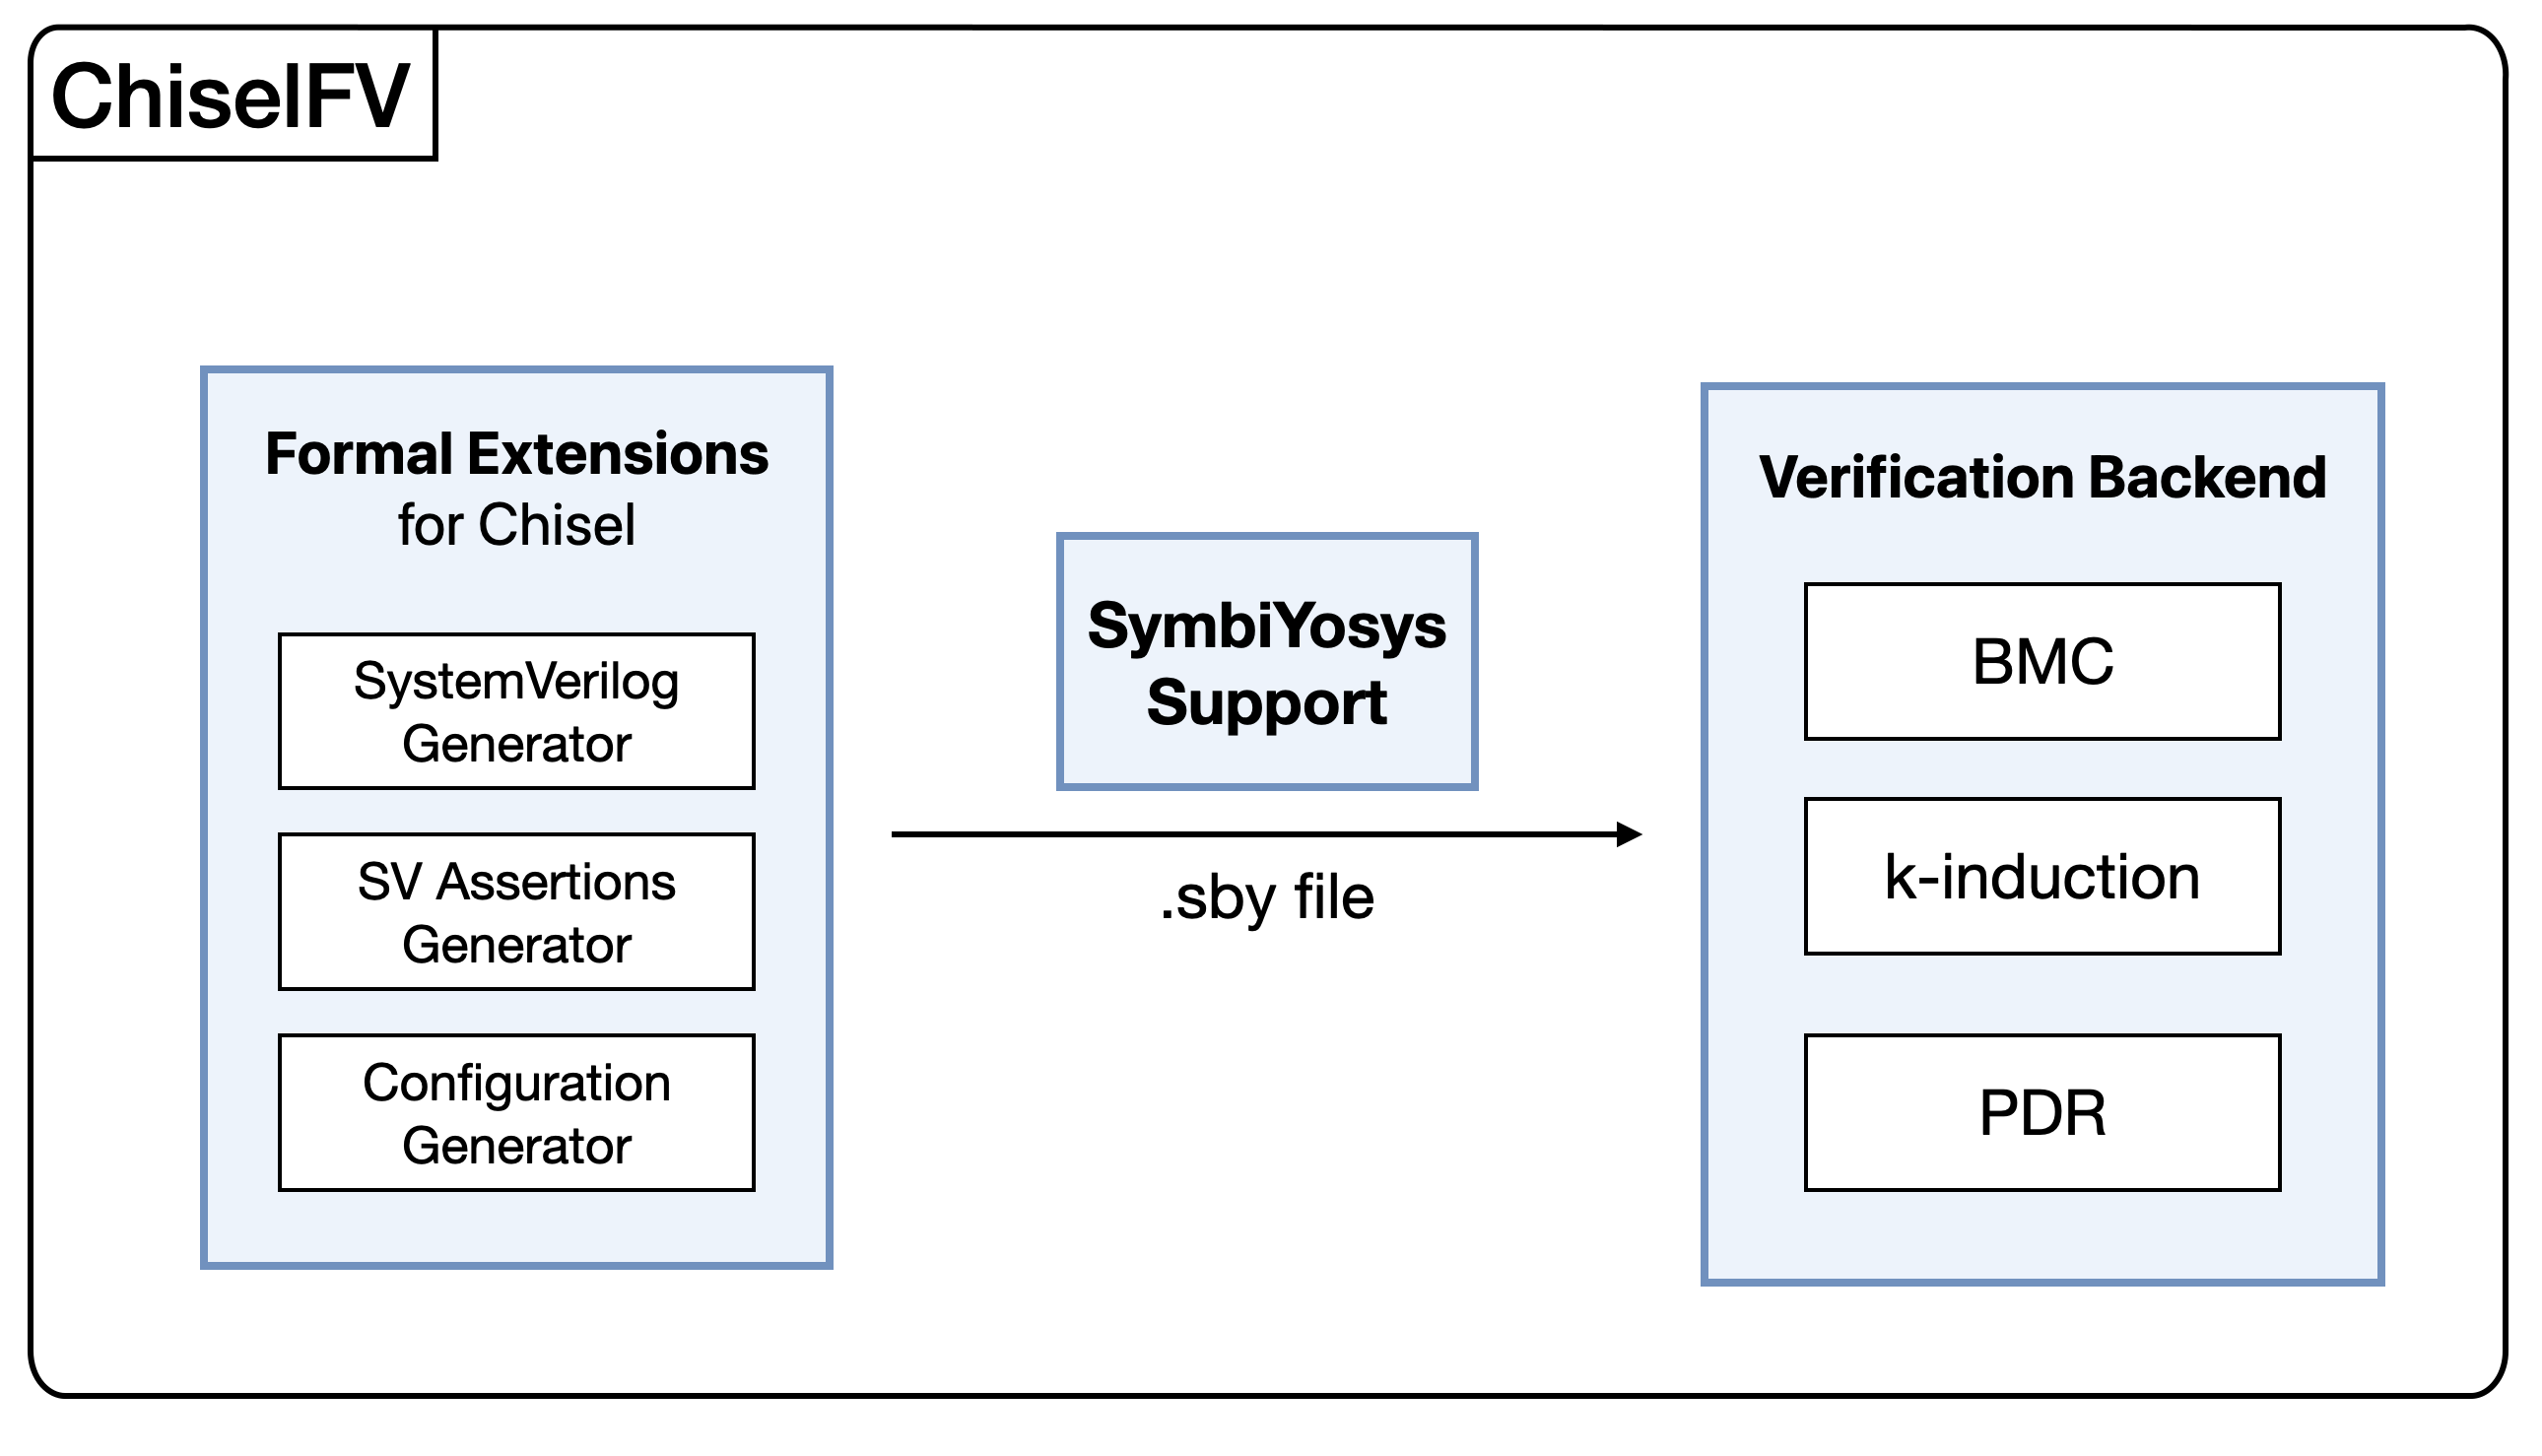
\includegraphics[width=1\linewidth]{pics/structure.png}
    \caption{ChiselFV Structure}
    \label{fig: structure}
    \end{center}
\end{figure}

As shown in Fig \ref{fig: structure}, ChiselFV is mainly an extension of Chisel's SystemVerilog generation and adds support for formal verification syntax. It also integrates the verification frontend and backend based on SymbiYosys, enabling one-key verification. The SystemVerilog generation is performed by calling the SystemVerilog generation process in Chisel. 
% 对于性质描述,ChiselFV 会将在 Chisel 定义的性质编译为 SVA 代码,对于复杂的性质描述,则会生成一些辅助电路来完成性质定义。
For property descriptions, ChiselFV compiles the properties defined in Chisel into SVA code. Some auxiliary circuits will be generated to complete the property definition for complex property descriptions.
And the configuration generator generates SymbiYosys-supported verification tasks configuration file .sby. 

Hardware developers can construct hardware modules in Chisel, and Chisel's compiler can compile Chisel modules to SystemVerilog code. The starting point of our work is to inject support for formal property descriptions in this stage.
Besides the SystemVerilog generation, we also add support for generating SystemVerilog Assertions and verification configuration files.

\begin{figure}[!htbp]
    \begin{center}
    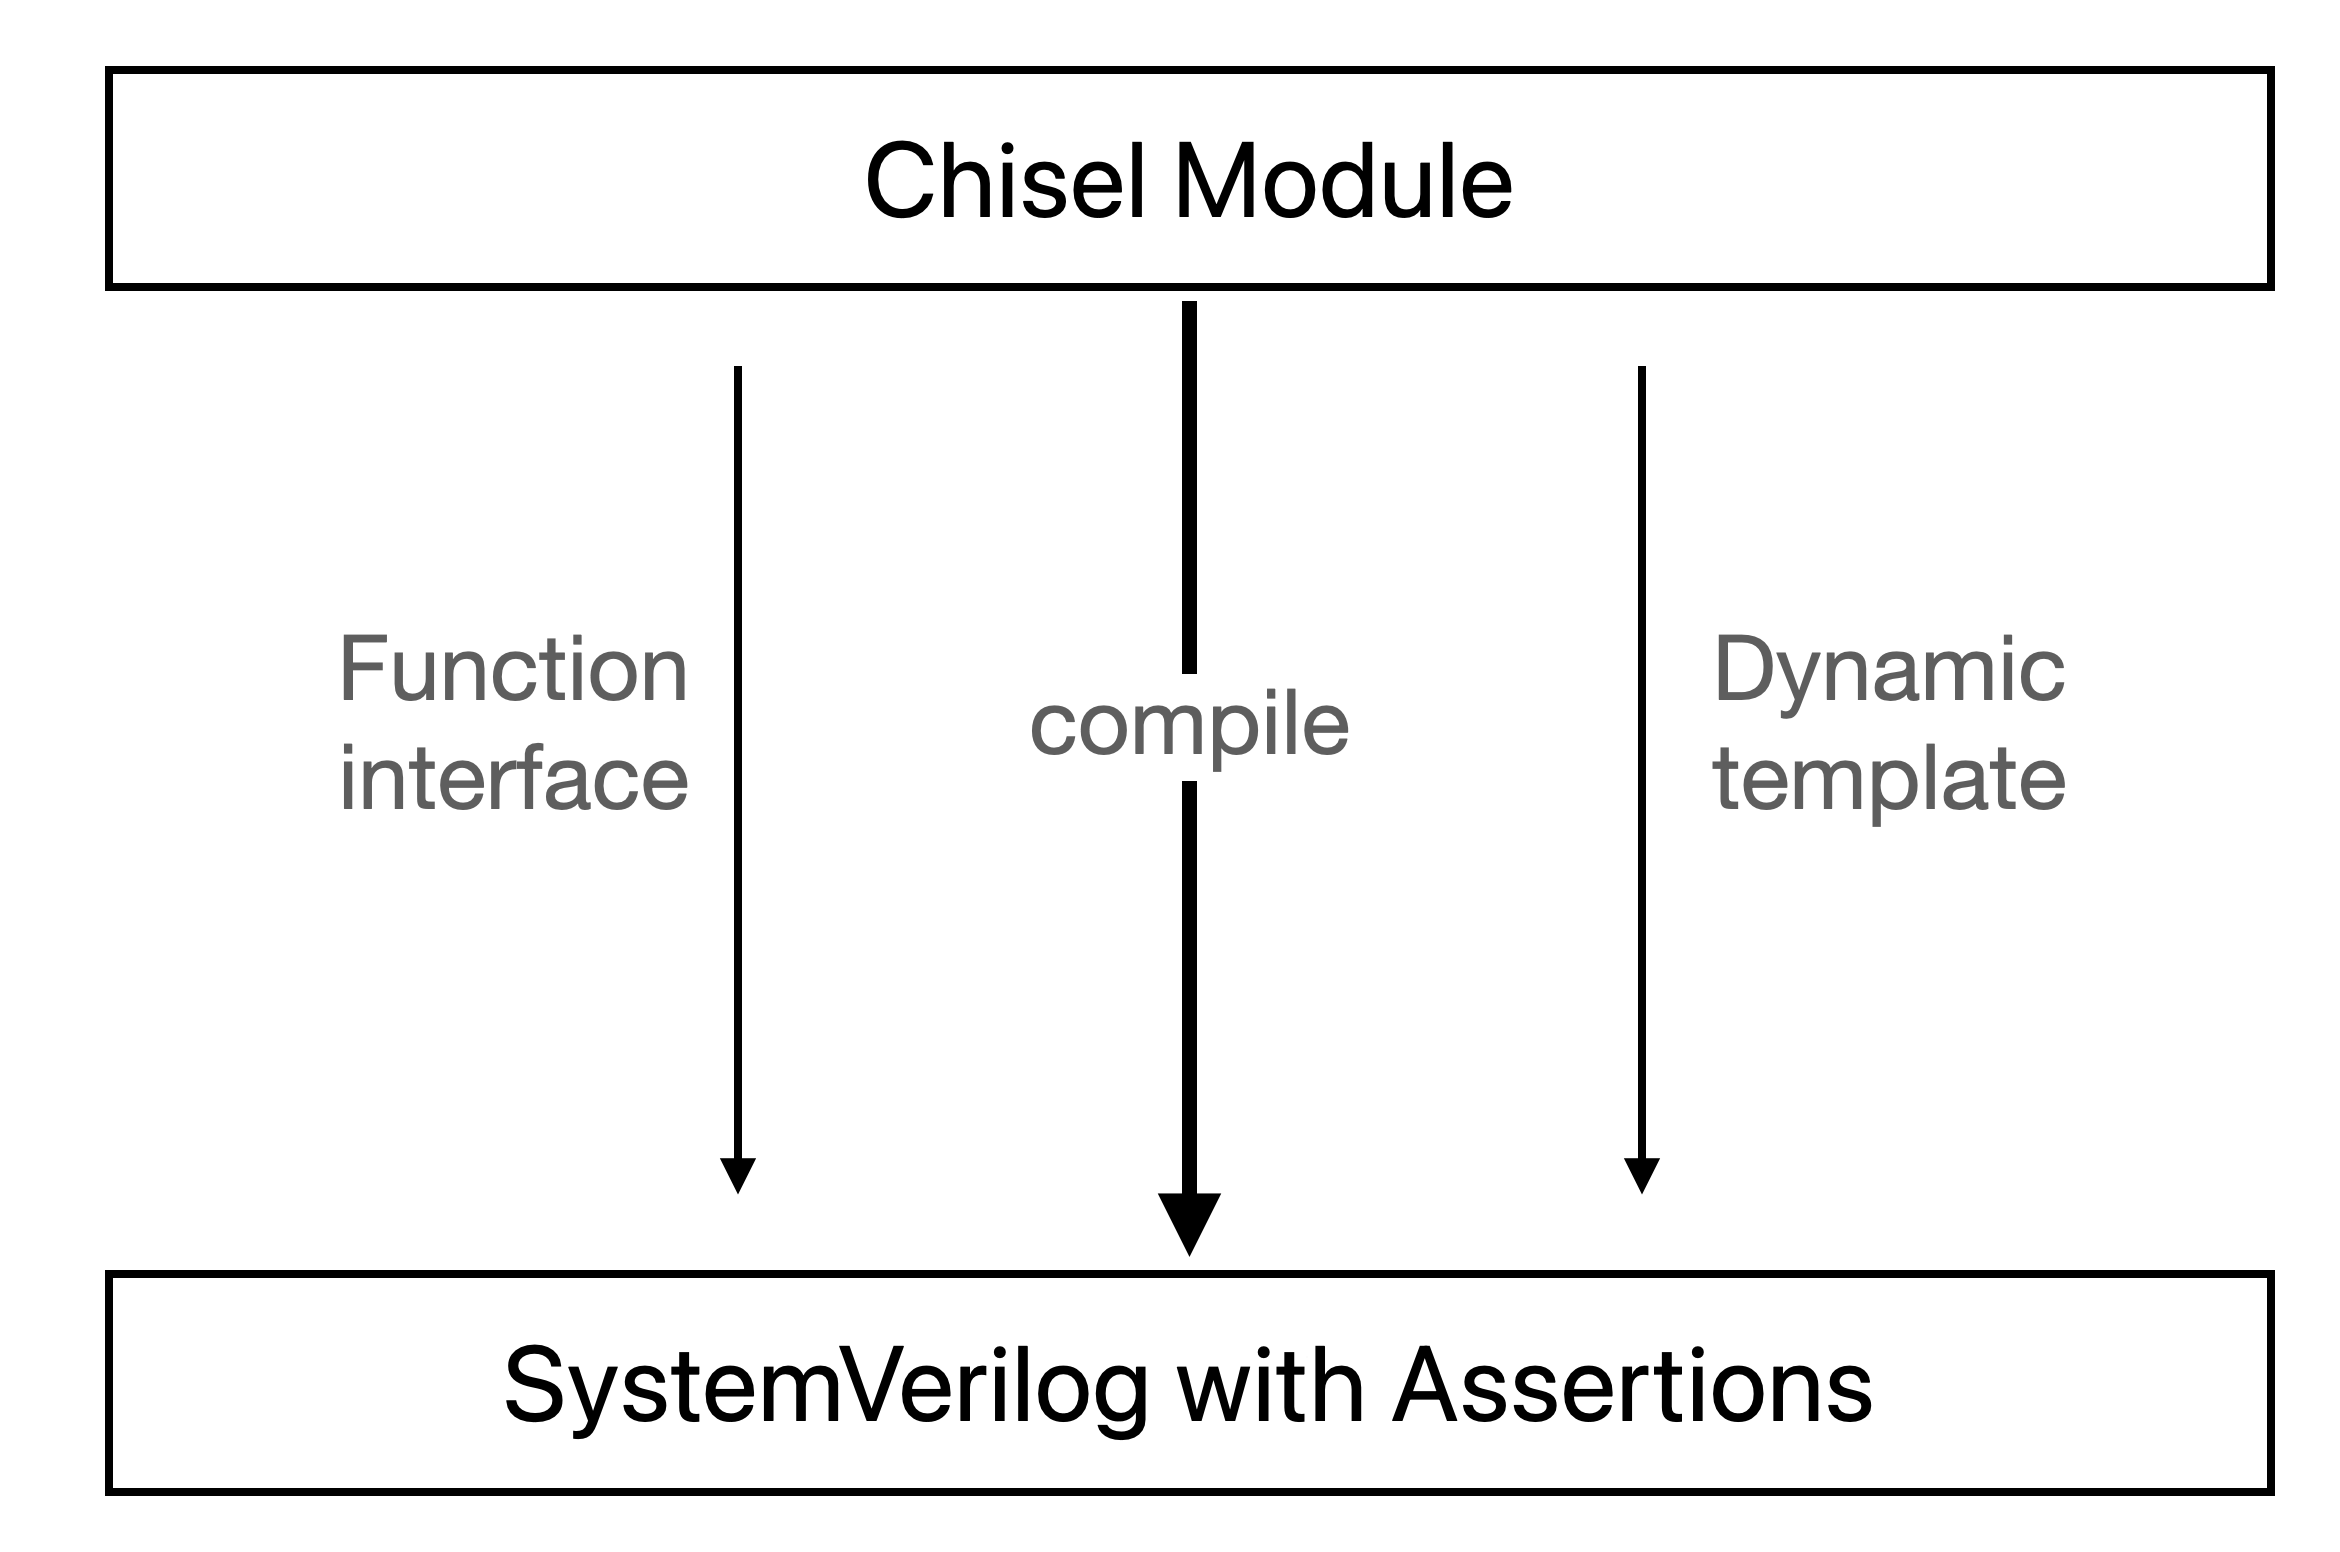
\includegraphics[width=0.9\linewidth]{pics/ChiselFVSubstitute.png}
    \caption{Technique in Chisel Compilation Extensions}
    \label{fig: ChiselFVSubstitute}
    \end{center}
\end{figure}

As shown in Fig \ref{fig: ChiselFVSubstitute}, we mainly use two techniques to extend the Chisel compilation process. The first is to use the Chisel hardware description abilities to implement the hardware code fragments equivalent to the property descriptions and encapsulate them into functions, providing an interface to call. This way, we implement a part of the formal property description syntax support.
% 例如后文中介绍的对于时序性质的支持,主要就是通过封装调用 Chisel 中提供的 \verb|ShiftRegister| 实例来实现的。
Such as to achieve the support for the temporal property description introduced in the following section, we mainly try to encapsulate the \verb|ShiftRegister| instance provided by Chisel into a function and provide an interface to call.

% 利用函数封装,提供接口的方式有一定的局限性,它要求保证性质的描述可以用 Chisel 提供的硬件描述能力来实现,而我们采用的第二种方式,动态模版,则是更加灵活。
Using function encapsulation and providing interfaces, there is a specific limitation, which needs to ensure that Chisel's hardware description abilities can implement the property description, and the second technique, dynamic template, is more flexible.
% 动态模版主要依赖于 Chisel 提供的 \verb|BlackBox| 类,通过编写 SystemVerilog 代码片段,并通过让其继承 \verb|BlackBox| 将其封装为一个新的 Chisel 模块,其将在 Chisel 模块编译时进行注入。同时在编写 SystemVerilog 片段时可以将外部的参数传入到该片段中,从而在编译时,模版会自动应用这些参数进行动态地实例化。
Dynamic template mainly depends on the \verb|BlackBox| class provided by Chisel. We write SystemVerilog code fragments and encapsulate them into a new Chisel module by inheriting \verb|BlackBox|, which will be injected into the Chisel module during compilation. At the same time, we can pass external parameters to the code fragment, and the template will automatically apply them to the instance dynamically during compilation.

% 最后,我们提供了验证配置文件的自动生成。
Finally, we provide the automatic generation of verification configuration files.
% ChiselFV 可以根据用户指定的验证方法和参数,生成对应的验证配置文件。这里主要采用了 sby 格式,它是由 SymbiYosys 支持。 ChiselFV 同时可以自动调用后端求解算法来根据具体的验证算法和参数,来对生成的模型进行验证。
ChiselFV can generate the corresponding verification configuration file according to the verification algorithm and parameters specified by the user. Here we use the .sby format, which is supported by SymbiYosys \cite{SymbiYosys}. ChiselFV can also automatically call the backend algorithm to verify the hardware model according to the specific verification algorithm and parameters.

\subsection{Formal Description Syntax}

% 下面我们给出在 ChiselFV 中支持的性质描述语法的定义。
We define the property description syntax supported by ChiselFV in Fig \ref{fig: syntax}.
The primary verification task in ChiselFV is: when the assumption defined in \verb|assume| block is true and whether the circuit assertion defined in \verb|assert| block is true or not. 

\begin{figure}[!htbp]
\begin{center}
\begin{equation*}
\begin{aligned}
    \langle \text{ChiselData} \rangle &::= \text{circuit node in Chisel} \\
    \langle \text{num} \rangle &::= \text{nonnegative integer} \\
    \langle \text{anyConst} \rangle &::= \text{circuit node with any constant value} \\ & \qquad \text{defined by Chisel extension support } \\
    \langle \text{valueExpr} \rangle &::= \text{past(} \langle \text{valueExpr} \rangle \text{, } \langle \text{num} \rangle \text{)} | \langle \text{ChiselData} \rangle \\ 
    & \qquad | \langle \text{anyConst} \rangle \\
    \langle \text{comparisonOp} \rangle &::= \text{`} \neq \text{'} \ | \text{`} = \text{'} \ | \ \text{`} < \text{'} \ |\ \text{`} \le \text{'} \ | \ \text{`} > \text{'} \ | \ \text{`} \ge \text{'}  \\
    \langle \text{logicalOp} \rangle &::= \text{`} \&\&\text{'} | \ \text{`} || \text{'} \\
    \langle \text{booleanExpr} \rangle &::=   \langle \text{valueExpr} \rangle \langle \text{comparisonOp} \rangle \langle \text{valueExpr} \rangle\\
    & \qquad |\langle \text{booleanExpr} \rangle \langle \text{logicalOp} \rangle \langle \text{booleanExpr} \rangle \\
    & \qquad | \text{`!'} \langle \text{booleanExpr} \rangle \\  
    & \qquad |  \text{`true.B'} | \text{`false.B'} \\
    \langle \text{assumption} \rangle &::= \text{assume(} \langle \text{booleanExpr} \rangle ) \\
    \langle \text{assertion} \rangle     &::= \text{assert(} \langle \text{booleanExpr} \rangle \text{)} \\
    & \qquad | \text{assertNextStepWhen(} \\ 
    & \langle \text{booleanExpr} \rangle \text{, } \langle \text{booleanExpr} \rangle \text{)} \\ 
    & \qquad | \text{assertAfterNStepWhen(} \\
    & \langle \text{booleanExpr} \rangle \text{, } \langle \text{num} \rangle \text{, } \langle \text {booleanExpr} \rangle \text{)} \\
    & \qquad | \text{assertAlwaysAfterNStep(} \\
    & \langle \text{booleanExpr} \rangle \text{, } \langle \text{num} \rangle \text{, } \langle \text {booleanExpr} \rangle \text{)} \\
\end{aligned}
\end{equation*}
\end{center}
\caption{Syntax of Property Descriptions}
\label{fig: syntax}
\end{figure}

% 对于电路的性质定义,基本上继承在 Chisel 中的语法,对于 Chisel 中返回值为 \verb|Bool| 的数据节点可以作为性质描述(定义为 \langle booleanExpr \rangle),它可以由数据变量之间的比较结果构成。
For the property definition, the basic syntax is inherited from Chisel. It means that the data nodes with return type \verb|Bool| in Chisel can be defined as property descriptions (defined as $\langle \text{booleanExpr} \rangle$ here), which can be constructed by the comparison results between data variables (defined as $\langle \text{valueExpr} \rangle$ here).

% 同时,我们还主要增强了对时序性质的描述支持,以及对自由常量的支持。接下来给出详细介绍。
In addition, we mainly enhance the description support for temporal properties and free constants. The following gives a detailed introduction.

\subsubsection{Immediate Assertions}
% ChiselFV 支持基本的断言类型。
ChiselFV supports the basic immediate assertion types.
% 在 ChiselFV 中,可以使用 |assume(expr)| 语法定义一个需要恒成立的假设,使用 |assert(expr)| 提供一个断言。
In ChiselFV, we can use the syntax \verb|assume(expr)| to define an assumption that must always be true, and use the syntax \verb|assert(expr)| to provide an assertion. The model checker will try to find a counter-example to the assertion or prove its correctness. Note that the search space is the circuit state after the first reset, i.e., without considering the Chaos before the first reset.
% \begin{itemize}
%   % assume(<expr>): 当进行形式化验证时,所以的 assumeptions 都假设为真,从而可以用于手动缩小验证模型系统的规模。其中 |<expr>| 可以是 Chisel 中的任意返回为 |Bool| 的表达式。
%   \item[a.] \verb|assume(expr)|: \\ When performing formal verification, all assumptions are assumed to be true and can be used to shrink the verification model. The expression \verb|expr| can be any expression in Chisel that returns a \verb|Bool|.
%   % assert(<expr>): 断言即在形式化验证时检查的内容,模型检查引擎会尝试找到令其为 False 的反例,或者证明其正确性。注意到这里搜寻的空间是电路在第一次复位后,即不去考虑复位前的 Chaos 状态。
%   \item[b.] \verb|assert(expr)|: \\ Assertions are checked during formal verification. The model checker will try to find a counter-example to the assertion or prove its correctness. Note that the search space is the circuit state after the first reset, i.e., without considering the Chaos before the first reset.
% \end{itemize}

% 时序性质定义
\subsubsection{Temporal Assertions} 
% ChiselFV 为时序相关的性质描述提供了丰富的支持。
ChiselFV provides rich support for temporal property descriptions.
\begin{itemize}
    % 可以使用 past 语句获取某个信号在 |<num>| 时刻之前的值。
    \item[a.] \verb|past(expr, num)|: \\ It can be used to get the value of a signal at time \verb|<num>| before the current time.
    \item[b.] \verb|assertAfterNStepWhen(cond, num, expr)|: \\ 
    It can be used to assume that when the \verb|cond| is true, the \verb|expr| signal is true in \verb|num| steps.
    % 在 SVA 语法中,类似于语句 |cond -> ##num expr|.
    In SVA syntax, it is similar to the statement \verb|cond -> ##num expr|.
    Additionally, \verb|assertNextStepWhen(cond, expr)| is equivalent to \verb|assertAfterNStepWhen(cond, 1, expr)|.
    \item[c.] \verb|assertAlwaysAfterNStep(cond, num, expr)|: \\
    It can be used to assume that when the \verb|cond| is true, the \verb|expr| is always true after \verb|num| steps. In SVA syntax, it is similar to the statement \verb|cond -> ##[num:] expr|.
\end{itemize}

\subsubsection{Universal Quantification}
% ChiselFV 提供了对于全称量词的支持。虽然在硬件电路中描述的是任意一个固定位长的数字,但是这仍然极大提高了对于性质的表达能力。在底层实现上,等价于一个类似于输入的节点,同时约束每个时刻保持值不变。在 ChiselFV 中可以调用 |anyconst(w)| 来得到一个任意位长为 |w| 的值。
In ChiselFV, we provide support for universal quantification. Although we describe a fixed-width number in hardware circuits, this still greatly improves the expressiveness of property description. In the implementation, we treat it as a node equivalent to an input node and constrain the same value at every clock cycle. In ChiselFV, we can call \verb|anyconst(w)| to get any value of fixed-width \verb|w|.

\subsection{Verification Engines}
In ChiselFV, we select three mainstreaming algorithms as backend engines: BMC \cite{biere1999symbolic}, k-induction \cite{sheeran2000checking} and PDR \cite{bradley2011sat} algorithm. 
% 他们都是依赖于 SAT / SMT 求解器的典型模型检测算法。经过 ChiselFV 的前端,将硬件设计和性质描述转化为了迁移系统,和迁移系统的待验证性质。BMC 算法主要通过验证模型在 k 步之内是否安全,它只能去尝试发现模型是否有错,而无法给出模型正确性的证明;K-induction 算法则是尝试证明待验证性质是否是 k 步归纳不变式;PDR 算法则是不断增强性质,企图得到一个一步归纳不变式。后两者都可能给出系统正确性的证据,并且可以发现错误。这三种算法各有优劣,BMC 算法 和 k-induction 比较直观简单,但是并不能解决所有问题,PDR 较为复杂,作为补充可以解决更多的问题。 
They are all typical model checking algorithms that rely on SAT/SMT solvers. After the front-end of ChiselFV, the hardware design and property definition are transformed into a transition system, and the property is to be verified. The BMC algorithm mainly verifies whether the model is safe within k steps. It can only try to find whether the model is wrong within some steps but cannot prove the correctness of the model. The k-induction algorithm tries to confirm that the property to be verified is an invariant of k steps. The PDR algorithm is to enhance the property step by step, trying to get an invariant of one step. The latter two may provide evidence of system correctness and can find errors. These three algorithms have their advantages and disadvantages. The BMC algorithm and k-induction are more intuitive and straightforward, but they cannot solve all problems. The PDR algorithm is more complex and can solve more problems as a supplement.

\begin{lstlisting}[language=scala, caption={A Code Clip to Call Formal Verification}, label=checker]
Check.kInduction(() => new Memory, 20)
\end{lstlisting}

% 在 ChiselFV 中,可以通过简单的一行代码来完成对验证算法的调用。如 Listing 1 所示,这段代码将会对 Memory 模块中的性质描述进行验证,使用 k-induction 算法运行 20 步。
In ChiselFV, we can call the verification engines with a simple line of code. As shown in Listing \ref{checker}, this code can verify the property defined in the Memory module using the k-induction algorithm for 20 steps.

% \begin{figure*}[!htbp]
%     \begin{center}
%     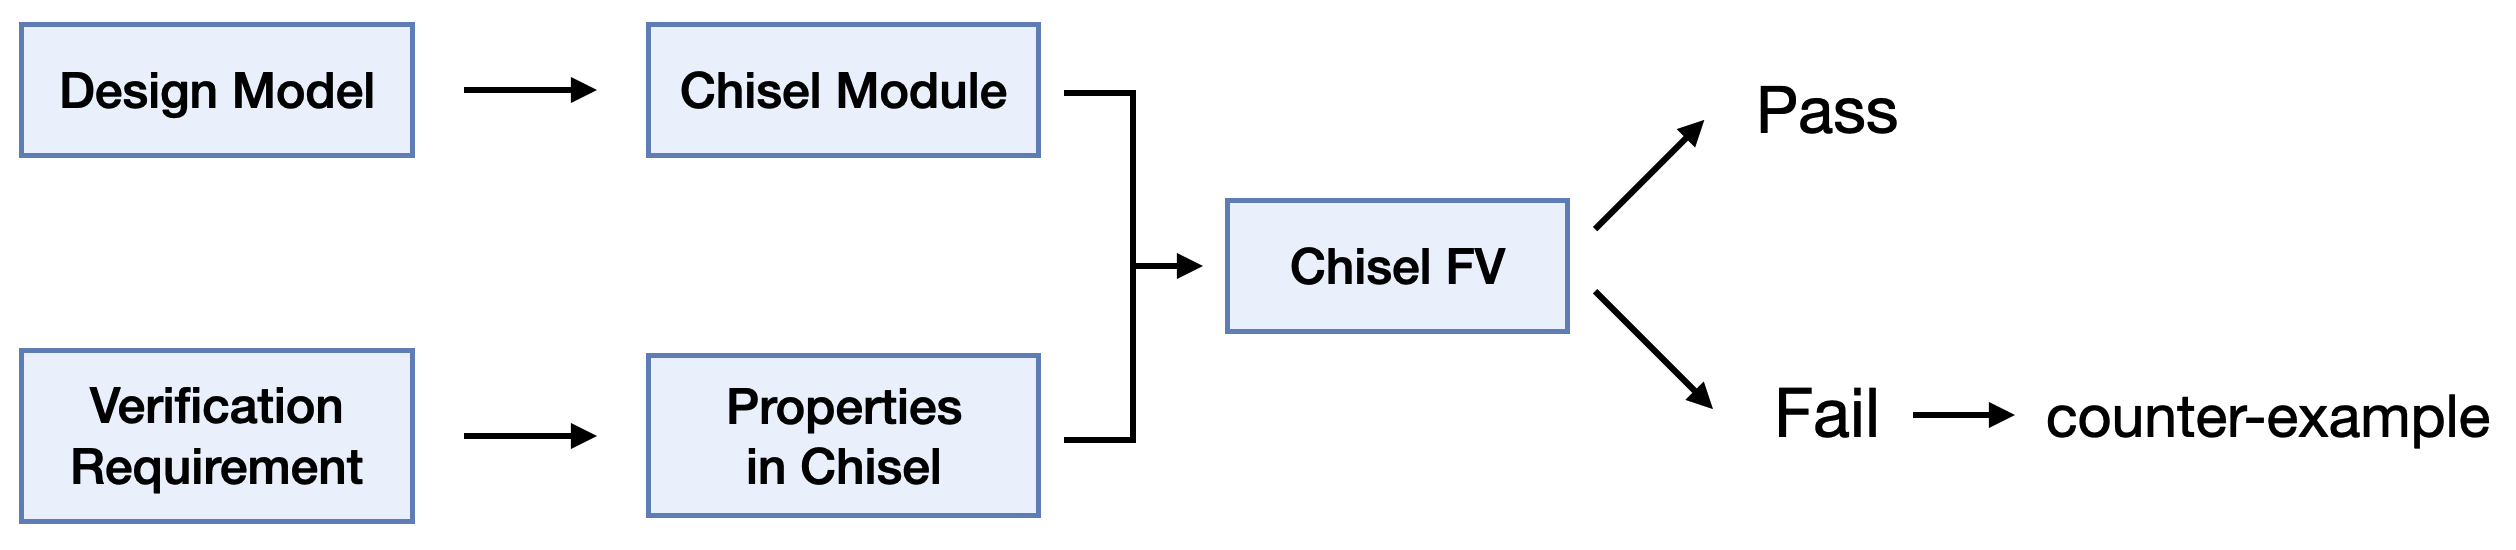
\includegraphics[width=0.8\linewidth]{pics/workflow.png}
%     \caption{Workflow of Designing and Formal Verifying a Circuit in Chisel with ChiselFV}
%     \label{fig: workflow}
%     \end{center}
% \end{figure*}

% 同时,ChiselFV 中的前端和后端引擎是分离的,使得后端有很好的扩展性。ChiselFV 支持更换不同的求解引擎,也可以对求解引擎中使用的 SAT/SMT 求解器进行更换。
At the same time, the front-end and back-end engines in ChiselFV are separated, which makes the back-end have good extensibility. ChiselFV supports replacing different engines and replacing the SAT/SMT solvers used.

\subsection{Methodology}

% 接下来我们来讨论在 Chisel 下设计实现并形式化验证电路的工作流,在 ChiselFV 帮助下。
Next, we discuss the workflow of designing and formal verifying a circuit in Chisel with the help of ChiselFV.

% 如图 \ref{fig: workflow} 所示,这个工作流的第一步是明确电路的设计需求,即需要分析清楚电路需要实现什么功能,进而可以将其作为我们的验证需求。同时需要做的是对电路的结构进行设计。
The first step of this workflow is to clarify the design requirements of the circuit, that is, to analyze what functions the circuit needs to implement, and then it can be used as our verification requirements. At the same time, we need to design the structure of the circuit.

% 接下来是使用 Chisel 来实现参数化的硬件模块,并使用上面提供的支持来将性质描述实现。这一步是比较关键的,也是最为困难的一步。本文中我们不去讨论如何使用 Chisel 来实现硬件模块,因为这不是我们的研究重点。但是如何将自然语言描述的性质,利用 ChiselFV 提供的性质描述语法来形式化表达出来,仍然是比较不容易的。一方面依赖于形式化验证工程师的经验,另一方面同时也有一些固定的套路和技巧。我们的 ChiselFV 提供了足够强大的形式化性质描述能力,可以在 Case Studies 章节中体会到。
Next, we use Chisel to implement the hardware module and the property description.
This is the most challenging step in the process. This paper does not discuss using Chisel to implement hardware modules because this is not our primary research focus. However, how formalizing the property description from natural language is still difficult.
On the one hand, it depends on the experience of formal verification engineers, and on the other hand, there are also some fixed patterns and tricks. Our ChiselFV provides sufficient formal property description capabilities, which will be more intuitive to show in the next section, Case Studies.

% 使用 ChiselFV 对性质进行描述之后,直接调用形式化求解的函数即可进行验证。由于在我们的验证框架中,仍然使用 SystemVerilog 和 SVAs 作为其中的一个中间形式,意味着验证的对象必须要被实例化。将实例化的对象直接传入需要的验证方法中即可调用验证过程,并获得验证结果。验证结果可能是失败,那么说明该性质在电路中会被违反,同时会给出反例;也可能是成功,代表该性质会始终成立;也有可能返回未知,对于当前性质,该算法引擎无能为力,可以考虑换一个求解引擎,或者修改性质表达。
After describing properties in ChiselFV, we can directly call the verification function to verify and get the result.
% Because we still use SystemVerilog and SVAs as the intermediate form in our verification framework, the object to be verified must be instantiated. 
% 我们可以调用验证方法并得到结果
% We can call the verification method and get the result. 
The result may be a failure, which means that the property is violated in the circuit, and we get a counter-example; 
it may be a success, which means that the property will always be true; 
it may be unknown, which means that the current algorithm engine cannot solve the property. We can consider changing the algorithm engine or modifying the property expression.

\section{Case Studies}

% 本节使用 ChiselFV 框架来形式化验证多端口内存和一个教科书中的典型五级流水设计。
This section uses the ChiselFV framework to make formal verification for multi-ported memory and a typical five-stage pipeline design in textbooks.

\subsection{Multi-ported Memory}

Multi-ported Memories are essential for high-performance parallel computation systems. VLIW and vector processors, CGRAs, DSPs, CMPs, and other processing systems often rely upon multi-ported memories for parallel access, hence higher performance \cite{abdelhadi2014modular}. 

However, implementing multi-ported Memory is quite expensive, so FPGA manufacturers often only provide dual-ported block memory, and hardware engineers need to use the existing dual-ported block memory to design multi-ported Memory. 
% The mainstream scheme is to use redundant dual-ported block memory, a two-dimensional block memory array, to implement multi-ported Memory, mainly divided into two classes. One class is based on using a small number of registers to store data, such as live-value-table (LVT) multi-ported Memory; another class is based on hiding the row number information in data, and the scheme is XOR-based multi-ported memory \cite{laforest2012multi}. 
Based on the previous work \cite{xiang2022parameterized}, we implement three high-parameterized multi-ported memories in Chisel, whose code can be found in GitHub repositories \cite{mpMemory}.
% Two of them are the ones we mentioned above, and the other is one-hot-encoding-based multi-ported Memory, whose code can be found in GitHub repositories \cite{mpMemory}.

\begin{figure}[!htbp]
    \begin{center}
    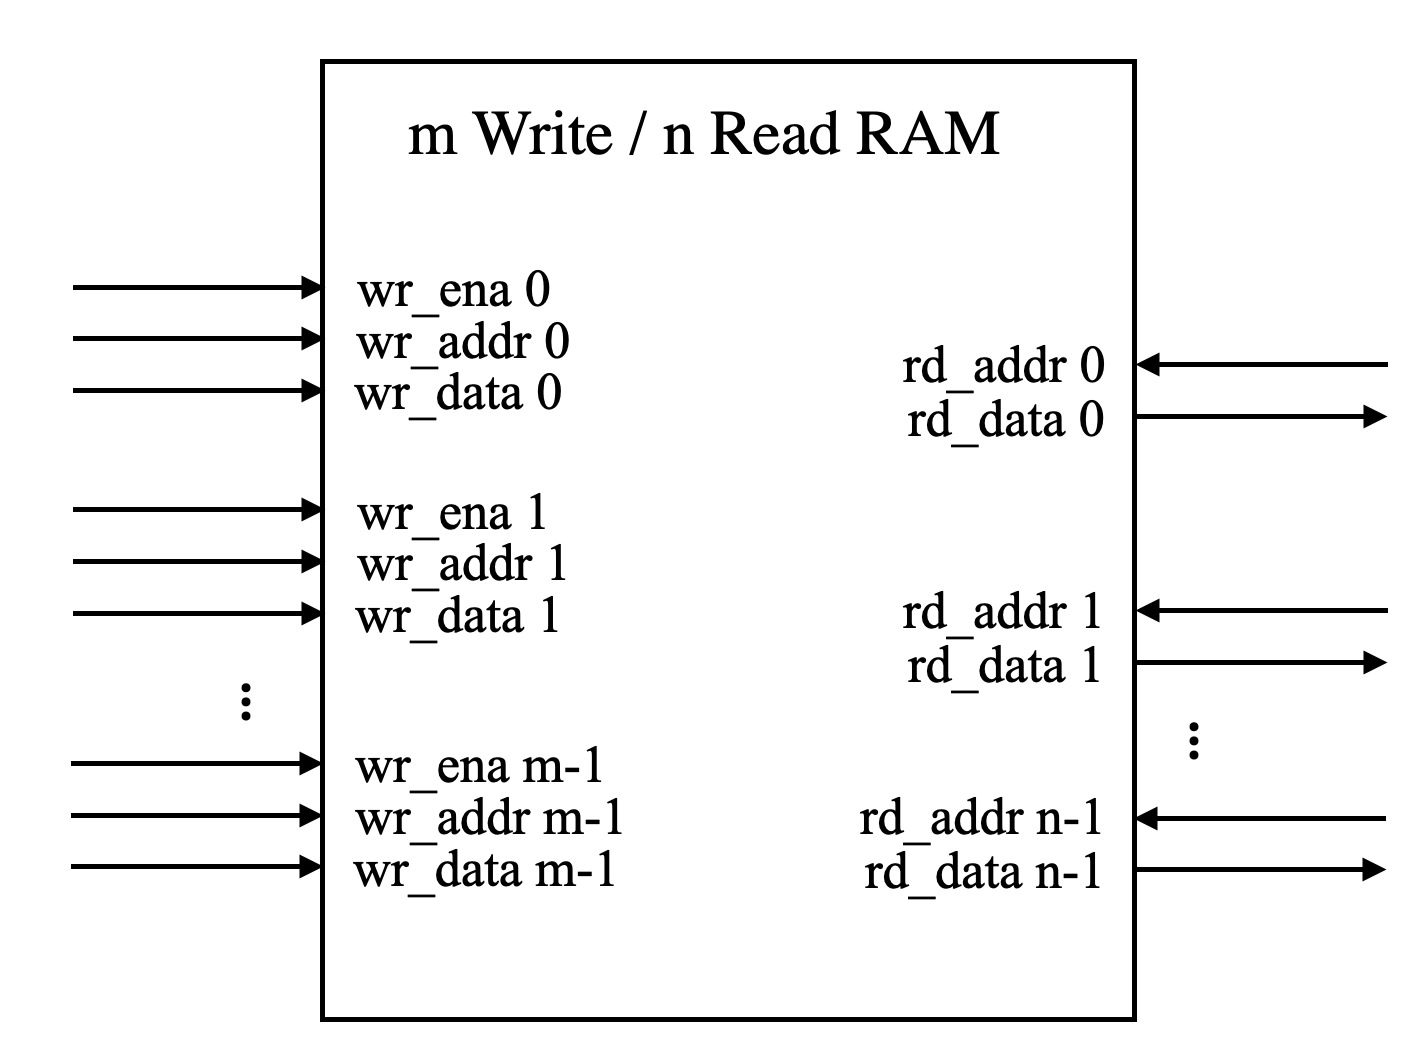
\includegraphics[width=0.9\linewidth]{pics/mpmemoryio.png}
    \caption{M write ports / N read ports Memory}
    \label{fig: mpmemoryio}
    \end{center}
\end{figure}

In this paper, our focus is not on the design itself, so we abstract the multi-ported Memory.
% We are concerned about whether the multi-ported Memory can meet our requirements, so its internal implementation can be shielded, and 
We are only concerned about its input and output. The basic IO of a multi-ported memory with m write ports and n read ports is shown in Fig \ref{fig: mpmemoryio}.

% 同时,我们需要设计验证需求,即我们需要多端口内存能够做到什么。可以通过 Fig 6 直观看到,性质可以描述为:
At the same time, we need to design the verification requirements, that is, what we need the multi-ported Memory to do. As shown in Fig \ref{fig: memverify}, the property can be described as: at any time, any write port $i$ can write $data_1$ to any address $addr$, and then after any time $t$, if there is no write operation to the same address during this period, $data_2$ read from the address should be the same as $data_1$.

\begin{figure}[!htbp]
    \begin{center}
    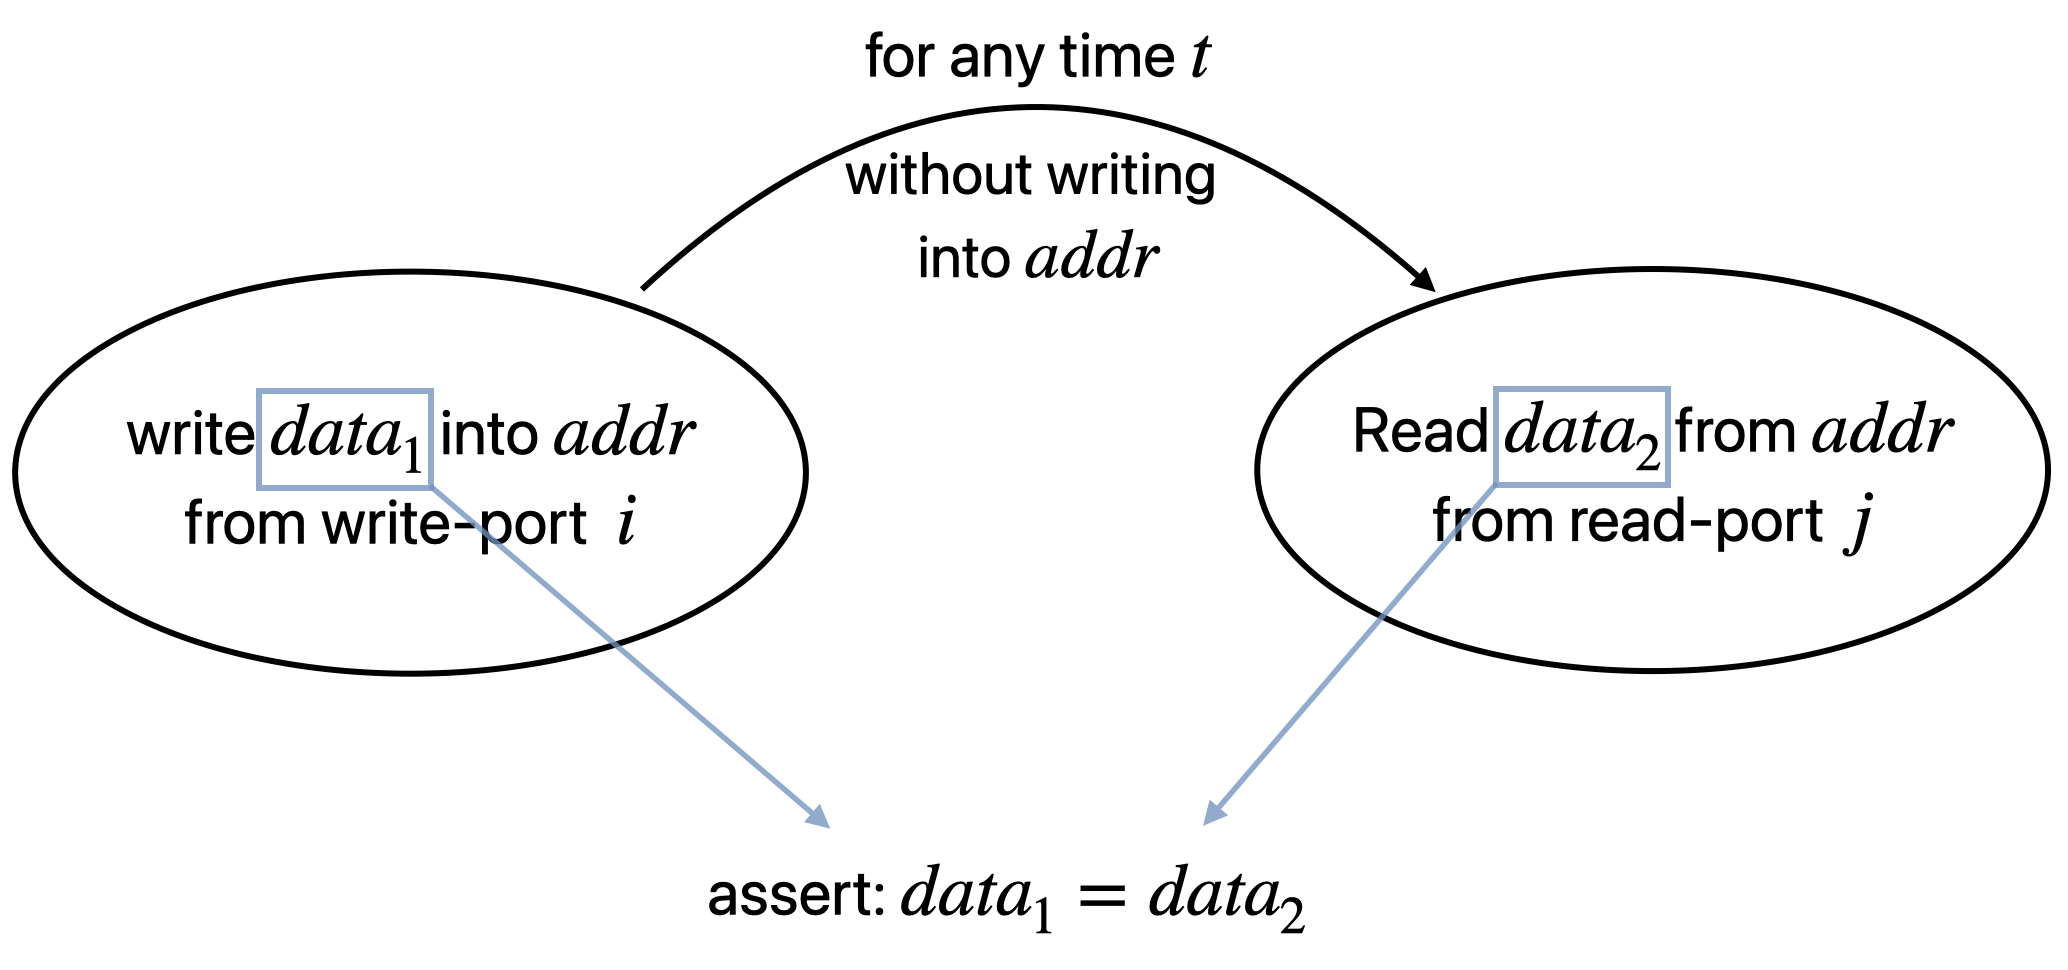
\includegraphics[width=1\linewidth]{pics/memverify.png}
    \caption{The property we need to verify in multi-ported memory}
    \label{fig: memverify}
    \end{center}
\end{figure}

% 接下来,需要使用 Chisel 对该模块进行实现,同时在 Chisel 上对性质进行定义。
Next, we need to implement the module in Chisel and define the property. 
% Chisel 实现在仓库中,性质定义可以在 ChiselFV 项目的案例文件夹中找到。
The Chisel implementation is in the repository \cite{mpMemory}, and the property definition can be found in the case folder of the ChiselFV project \cite{ChiselFV}.
% 在这里,需要使用 |anyconst| 关键字构造一个任意值的 $addr$,使用一个寄存器 $data$ 存储写入 $mem_{addr}$ 的值。每当任意写端口对 $addr$ 地址发生写入时,将写入的值记录到寄存器 $data$ 中,每当任意读端口对 $addr$ 地址发生读入时,断言读出的结果和 $data$ 中的值相同。
Here, we need to use the \verb|anyconst| keyword to construct an arbitrary value of $addr$ and a register $data$ to store the value written to $mem_{addr}$. Whenever any write port writes to the $addr$ address, the written value is recorded in the register $data$, and whenever any read port reads from the $addr$ address, the read result is asserted to be the same as the value in $data$.
% 简化了的对性质定义代码如 Listing 2 所示。其中还需要去增加上对不同端口不会同时对 addr 写入的假设。
The simplified code for the property definition is shown in Listing \ref{memassert}. It is necessary to add the assumption that different ports do not write to $addr$ simultaneously.
% 模型和性质通过 k-induction 算法在 5 步内很快得到证明,详细代码在仓库中。
The k-induction algorithm, within five steps, quickly proves the model and property, and the detailed code is in the repository.

\begin{lstlisting}[language=scala, caption={Verification Code of Multi-ported Memory Module}, label=memassert]
val addr = anyconst(addrW)
val data = Reg(UInt(w.W))
for (i <- 0 until m) {
    when(io.wrAddr(i) === addr && io.wrEna(i) === true.B) {
        data := io.wrData(i)
    }
}
for (i <- 0 until n) {
    when(io.rdAddr(i) === addr && hasWritten) {
        assert(io.rdData(i) === data)
    }
}
\end{lstlisting}

\subsection{Five-stage Pipeline}
% 在经典的体系结构教科书中给出了一个简单五级流水线。
In the classic architecture textbooks \cite{patterson2017computer}, a simple five-stage pipeline is given. 
% 这个处理器设计有五级流水,分别为取指、译码、执行、访存、写回。
This processor design has five pipeline stages: instruction fetch and decode, execution, memory access, and write back. 
% 它实现了 RISC-V 指令集中的 |ld|,|sd|, |add|, |beq| 四个典型指令。
It implements four typical instructions in the RISC-V instruction set, including \verb|ld|, \verb|sd|, \verb|add|, and \verb|beq|.
% 通过转发和 stalling 的方式来避免数据冒险,在分支预测上,采取假定分支不会被采用的方式来处理控制冒险,如果预测错误,则会在中间插入一条 |nop| 指令来使得流水线保持正确。
It avoids data hazards by forwarding and stalling. On branch prediction, it adopts the way of assuming that the branch will not be taken to handle control hazards. If the prediction is wrong, a \verb|nop| instruction will be inserted in the middle to keep the pipeline correct.
% 书中采用 Verilog 语言对该处理器进行了具体的实现。在我们的工作中,我们首先使用 Chisel 实现了处理器,然后使用 ChiselFV 框架对其进行了形式化验证,实现和验证的代码都在 GitHub 仓库中。
The book uses the Verilog language to implement the processor. In our work, we first use Chisel to implement the processor and then use the ChiselFV framework to verify it formally. The implementation and verification code are in the GitHub repository \cite{riscvFvChisel}.

% 我们的验证方案主要受启发于 RISC-V Formal Verification Framework,他们是在 SystemVerilog 层次上提供了一套验证 RISC-V 处理器的框架,使用 SVA 定义性质,然后利用验证工具进行验证。
Our verification solution is mainly inspired by the RISC-V Formal Verification Framework \cite{riscv-formal}. They provide a framework for verifying RISC-V processors at the SystemVerilog level, using SVA to define properties and then using verification tools to verify them.
% 我们尝试将 RISC-V Formal 验证框架利用 ChiselFV 迁移到 Chisel 层次,从而实现对 RISC-V 处理器的形式化验证。
We try to migrate the RISC-V Formal verification framework to the Chisel level by ChiselFV to verify the RISC-V processor at the Chisel level.

% Chisel 版本 RISC-V Formal 框架图
\begin{figure}[!htbp]
    \begin{center}
    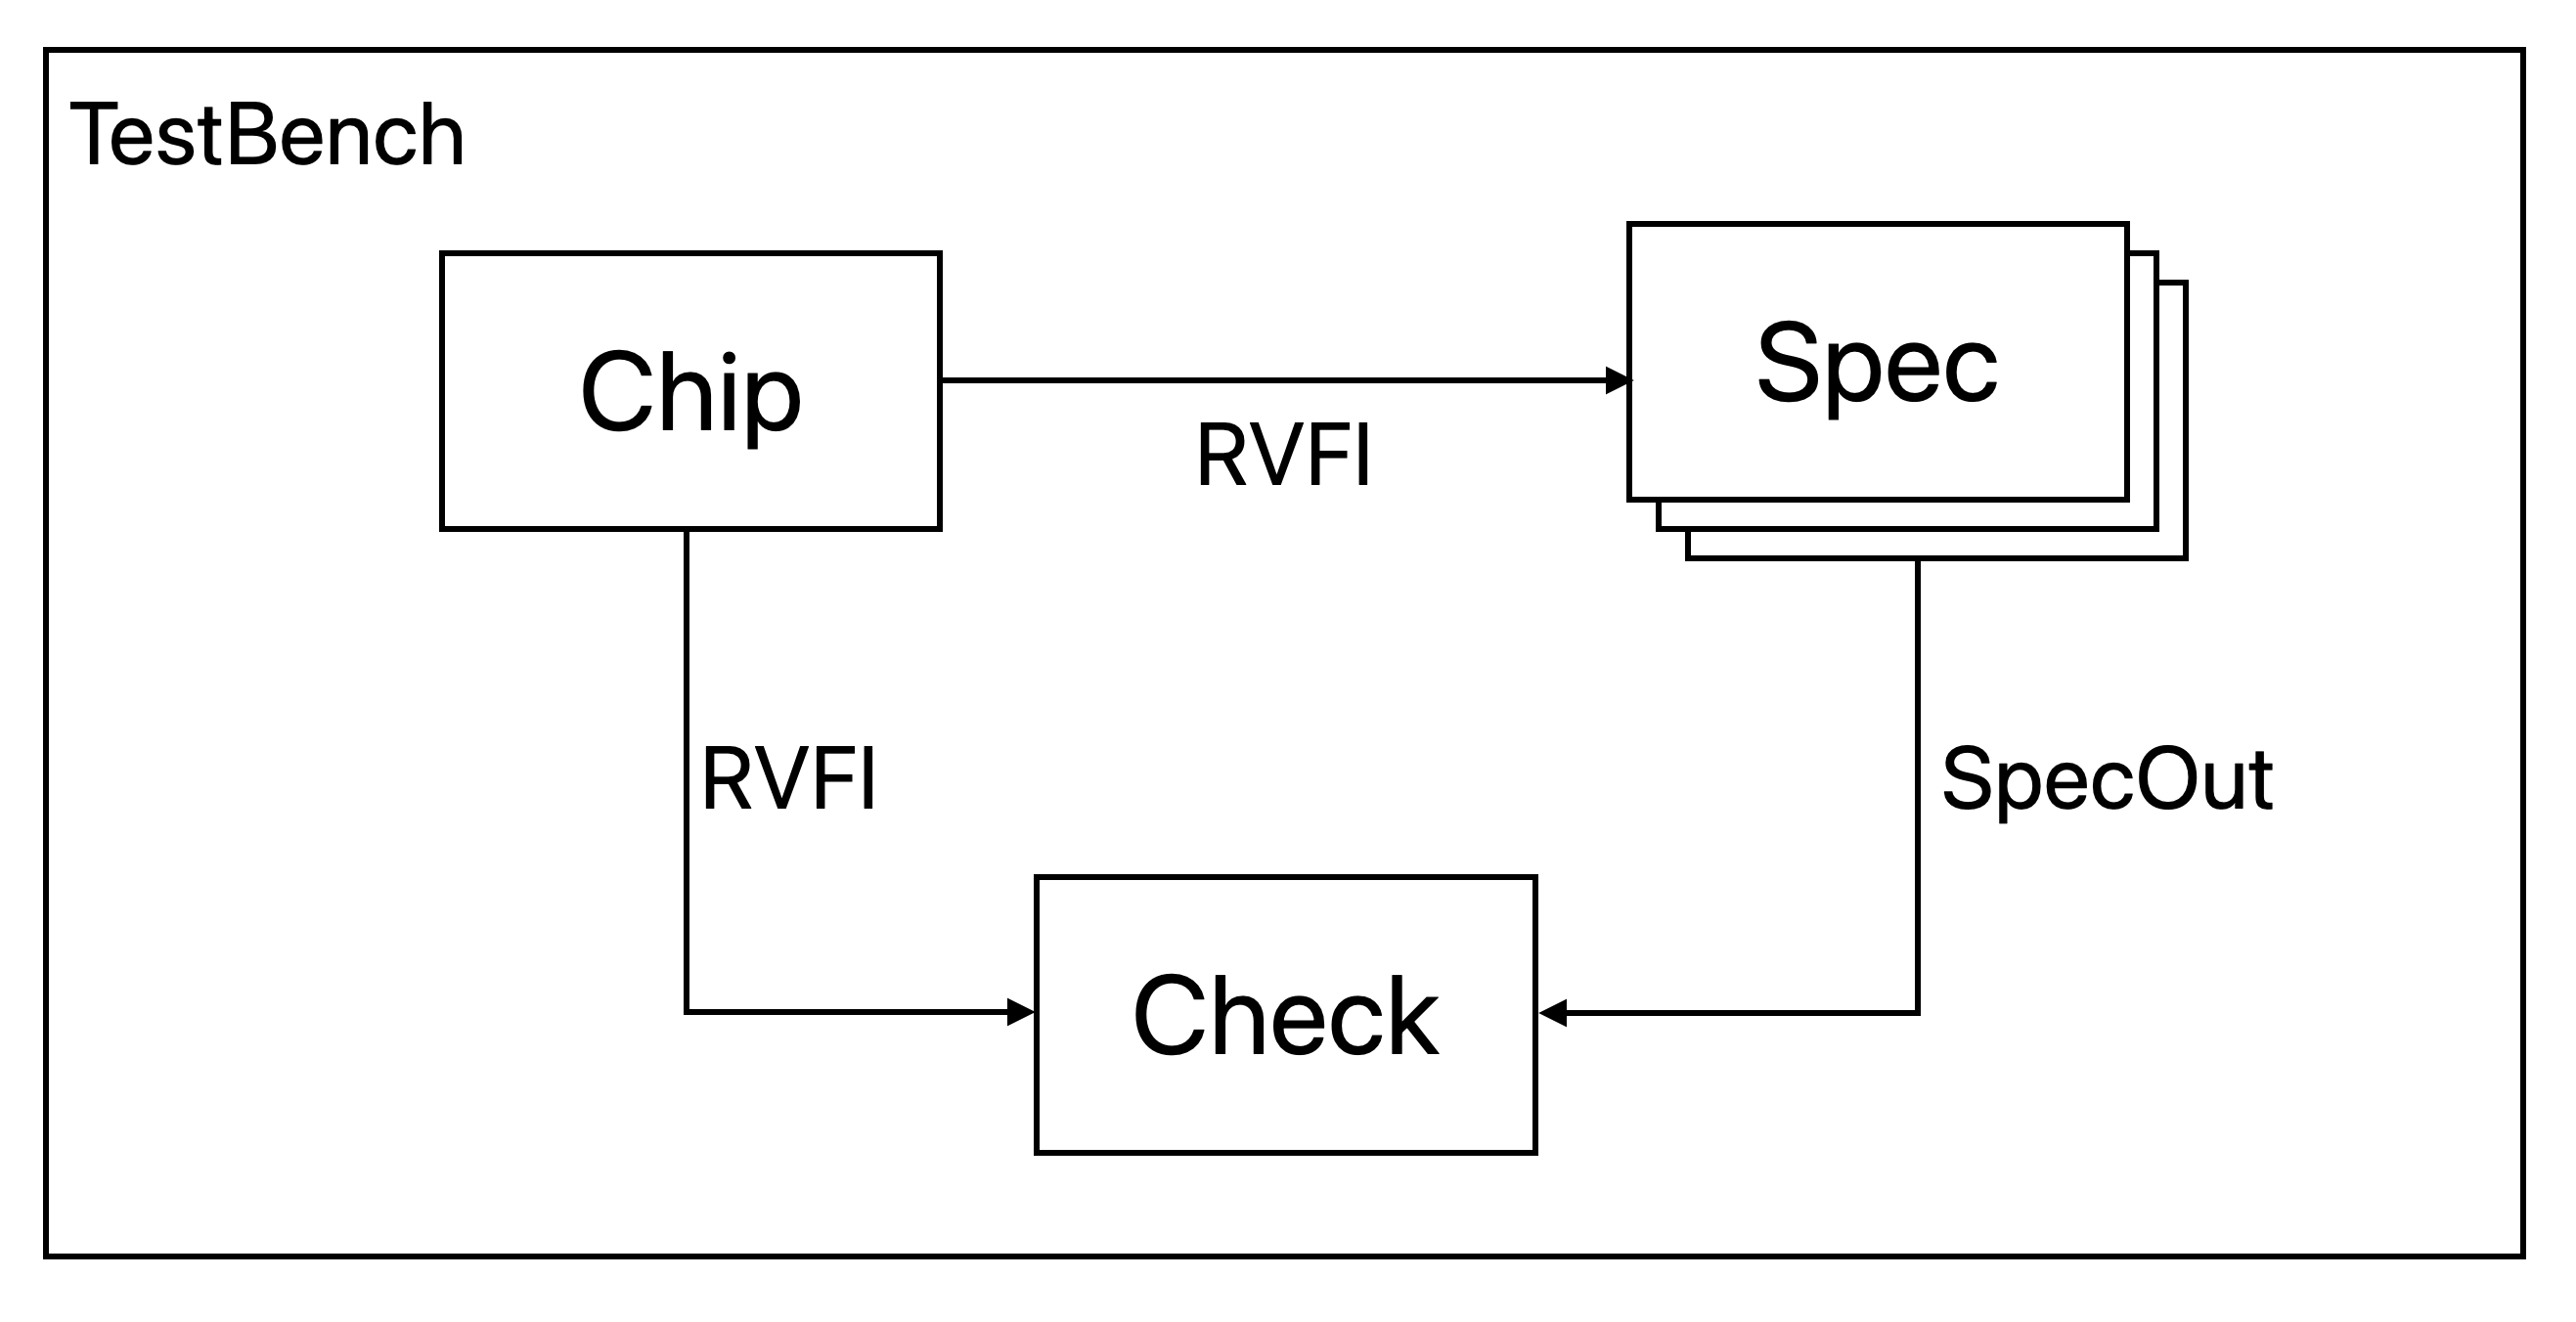
\includegraphics[width=1\linewidth]{pics/riscvFvChisel.png}
    \caption{Chisel Version RISC-V Formal Verification Framework}
    \label{fig: riscvFv}
    \end{center}
\end{figure}

% 验证方案方案如图 7 所示,流水线处理器实现在 Chip 模块中,Chip 模块需要向外提供 RVFI 接口,输出每条指令执行过程中的关键信息。
The verification solution is shown in Figure \ref{fig: riscvFv}. The pipeline processor is implemented in the Chip module, and the Chip module needs to provide the RISC-V Formal Interface (RVFI) to output the critical information of each instruction execution process. 

% RVFI 接口定义如 Listing 3 所示。
The RVFI interface definition is shown in Listing \ref{rvfiio}.
% 对于每条指令,拿到其指令的内容,解码的结果,执行前后 PC 寄存器的更新,源操作数,目标操作数,以及指令执行前寄存器的状态。
For each instruction, we get its instruction content, decoding result, PC register update before and after execution, source operands, destination operands, and register state before instruction execution.
% 从 Chip 中提取出 RVFI 是验证实现中关键的一步,需要使用 ChiselFV 中提供的时序能力来获取每条指令的执行过程中的信息,在执行完成时同时进行输出。
Extracting RVFI from Chip is a crucial step in the verification implementation. We need to use the temporal ability provided by ChiselFV to get the information of each instruction execution process and output it simultaneously when the execution is completed.

% RVFI 定义
\begin{lstlisting}[language=scala, caption={RVFI Definition}, label=rvfiio]
class RVFI_IO extends Bundle {
    val valid     = Output(Bool())
    val insn      = Output(UInt(32.W))
    val pc_rdata  = Output(UInt(64.W))
    val pc_wdata  = Output(UInt(64.W))
    val rs1_addr  = Output(UInt(5.W))
    val rs2_addr  = Output(UInt(5.W))
    val rs1_rdata = Output(UInt(64.W))
    val rs2_rdata = Output(UInt(64.W))
    val rd_addr   = Output(UInt(5.W))
    val rd_wdata  = Output(UInt(64.W))
    val mem_addr  = Output(UInt(32.W))
    val mem_rdata = Output(UInt(64.W))
    val mem_wdata = Output(UInt(64.W))
    val regs      = Vec(32, Output(UInt(64.W)))
}
\end{lstlisting}

% 接下来,需要定义 Spec 模块和 Check 模块。对于每个需要验证的指令实现或者小的性质,都可以通过单独一个 Check 来描述,其输入为 RVFI,通过对 RVFI 信号的分析,得出指令执行后正确的状态信息,通过 SpecOut 接口输出。定义 Check 模块,输入为来自 Chip 的 RVFI 和 来自某个 Spec 的 SpecOut,断言两份信号的一致性,从而对处理器的各个指令执行正确性进行验证。
Next, we need to define the Spec module and Check modules. For each instruction or small property that needs to be verified, a separate Check module can be 
Its input is RVFI, and its output is SpecOut, which is the correct state information after the instruction execution. Define the Check module, the input is RVFI from the Chip and SpecOut from some Spec, and assert the consistency of the two signals to verify the correctness of the execution of each instruction of the processor.
% 在目前的版本中,我们实现了对 |add|、|ld|、|beq| 指令执行功能正确性的验证。
In the current version, we have verified the correctness of the execution of the \verb|add|, \verb|ld|, and \verb|beq| instructions.
% 具体的验证设计在 GitHub 仓库中可以找到。
The specific verification design can be found in the GitHub repository.

% 最终,我们发现了该处理器在设计上有一个错误。ChiselFV 给出了一个执行会发生错误的执行路径。对于 |beq| 指令,需要比较两个源操作数的大小,但是在原来的设计中,这两个源操作数并没有考虑到数据冒险,而是直接从寄存器中拿到的数据,这是不合理的。之后,我们在 Chisel 版本上修改了设计,并通过了相关的验证。
Eventually, we found that there was an error in the design of this processor. 
As shown in Table \ref{ctx}
ChiselFV gives an execution path that would fail. For the \verb|beq| instruction, we need to compare the value of the two source operands, but in the original design, these two source operands were not considered data hazards. 
Instead, they were directly taken from the register. Later, we modified the design on the Chisel version and passed the relevant verification.

% ChiselFV 输出的反例
\begin{table}[!h]
    \caption{ChiselFV Output Counterexample}
    \label{ctx}
    \begin{tabular}{|l|l|l|l|}
    \hline
    \textbf{binary} & \textbf{instruction} & \textbf{PC} & \textbf{related regs}                                                                             \\ \hline
    0x00000013      & NOP                  & 0xFFFFFFFC  & \begin{tabular}[c]{@{}l@{}}x17: 0\\ x20: 0\end{tabular}                               \\ \hline
    0x0000F883      & ld x17, 0(x1)        & 0x0         & \begin{tabular}[c]{@{}l@{}}x17: 0x80000001\\ x20: 0\end{tabular}                      \\ \hline
    0x00508A83      & ld x21, 5(x1)        & 0x4         & \begin{tabular}[c]{@{}l@{}}x17: 0x80000001\\ x20: 0\end{tabular}                      \\ \hline
    0x00108C93      & addi x25, x1, 1      & 0x8         & \begin{tabular}[c]{@{}l@{}}x17: 0x80000001\\ x20: 0\end{tabular}                      \\ \hline
    0x03488063      & beq x17, x20, 32     & 0xC         & \begin{tabular}[c]{@{}l@{}}x17: 0x80000001\\ x20: 0\\ wrong branch taken\end{tabular} \\ \hline
    0x00000013      & NOP                  & -           & \begin{tabular}[c]{@{}l@{}}x17: 0x80000001\\ x20: 0\end{tabular}                      \\ \hline
    0xFC108AE3      & -                    & 0x2C        & \begin{tabular}[c]{@{}l@{}}x17: 0x80000001\\ x20: 0\end{tabular}                      \\ \hline
\end{tabular}
\end{table}
% \begin{table}[htbp]
% \caption{Table Type Styles}
% \begin{center}
% \begin{tabular}{|c|c|c|c|}
% \hline
% \textbf{Table}&\multicolumn{3}{|c|}{\textbf{Table Column Head}} \\
% \cline{2-4} 
% \textbf{Head} & \textbf{\textit{Table column subhead}}& \textbf{\textit{Subhead}}& \textbf{\textit{Subhead}} \\
% \hline
% copy& More table copy$^{\mathrm{a}}$& &  \\
% \hline
% \multicolumn{4}{l}{$^{\mathrm{a}}$Sample of a Table footnote.}
% \end{tabular}
% \label{tab1}
% \end{center}
% \end{table}


\section{Related Work}
This section presents a brief overview of the formal verification in hardware.

% 硬件形式化验证主要采用模型检测的方法。
Formal verification of hardware mainly uses model checking.
% Formal verification is divided into two directions: Theorem Proving \cite{Hoare69}, and Model Checking \cite{clarke2018handbook}. Theorem Proving relies on high-order logic and uses mathematical structures to build formulas corresponding to the system. And the verification process is the evaluation of these formulas. However, it isn't easy to automate. This means that the verification process needs to be assisted by engineers.
Model Checking is a method that can be fully automated but has a state explosion problem. To counter this problem, new technologies are introduced to reduce the state space of the transition system.

At the turn of the last century, a new generation of Boolean satisfiability (SAT) solvers such as Chaff \cite{MoskewiczMZZM01} brought about a leap in the performance and scalability of satisfiability checkers for propositional formulas. The hardware model checking technique particularly benefited from the advances of SAT solvers \cite{vizel2015boolean}. At the same time, Satisfiability Modulo Theories (SMT) \cite{barrett2018satisfiability} has also been rapidly evolving. 

Therefore, many model checking algorithms based on SAT/SMT solvers have been widely applied in hardware verification, such as BMC \cite{BiereCCZ99}, k-induction \cite{tinelli2012smt}, IC3/PDR \cite{Bradley11}, etc.

Besides the algorithms, the 
% easy-to-use, scalable, high-performance, and available in industrial environments 
hardware model checking tools are also an important research direction. Aina Niemetz, Clifford Wolf's work \cite{niemetz2018btor2} proposed BtorMC, a model checker built on Boolector. BtorMC supports the format Btor2, a new word-level model checking and witness format also proposed by them. Pono, a flexible and extensible SMT-based model checker, is designed to be both a research platform for developing and improving model checking algorithms and a performance-competitive tool that can be used for academic and industry verification applications \cite{mann2021pono}. It supports the verification format Btor2 and SMV. SymbiYosys is an open-source frontend driver program for Yosys-based formal hardware verification flow \cite{SymbiYosys}, and its team has already released a commercial EDA tool for hardware verification, Tabby CAD Suite. SymbiYosys supports direct verification of assertions in SystemVerilog. 
% 在第一章中详细说明的 ChiselVerify 和 Chisel 的形式化支持都是在 Chisel 层次做的验证工作。
ChiselVerify \cite{dobis2021chiselverify} and Chisel's formal support \cite{dobis2021open}, detailed in Chapter I, are both verification work at the Chisel level.

\section{Conclusion and Future Work}

In this paper, we introduce ChiselFV, a formal verification framework for Chisel. ChiselFV provides a workflow for formal verification of Chisel modules, which can be combined with Chisel-based hardware design development to significantly improve the efficiency and simplicity of hardware development and verification. ChiselFV provides strong property description support, which enables verification work previously done at the low-level RTL level, but can be done in Chisel, improving the level of hardware verification.

In the future, we will provide more advanced support for Chisel's formal verification. Currently, our verification backend is to convert it to SVAs and then perform the verification process. This means we cannot symbolize the module's parameters in Chisel and must instantiate it before verification. We will further develop a verification backend for Chisel, which will be able to symbolize the parameters of the modules for formal verification. We are also actively researching new verification algorithms, which we hope to develop into high-efficiency verification algorithms and integrate into ChiselFV.

% \begin{table}[htbp]
% \caption{Table Type Styles}
% \begin{center}
% \begin{tabular}{|c|c|c|c|}
% \hline
% \textbf{Table}&\multicolumn{3}{|c|}{\textbf{Table Column Head}} \\
% \cline{2-4} 
% \textbf{Head} & \textbf{\textit{Table column subhead}}& \textbf{\textit{Subhead}}& \textbf{\textit{Subhead}} \\
% \hline
% copy& More table copy$^{\mathrm{a}}$& &  \\
% \hline
% \multicolumn{4}{l}{$^{\mathrm{a}}$Sample of a Table footnote.}
% \end{tabular}
% \label{tab1}
% \end{center}
% \end{table}

% \begin{figure}[htbp]
% \centerline{\includegraphics{fig1.png}}
% \caption{Example of a figure caption.}
% \label{fig}
% \end{figure}


\bibliographystyle{IEEEtran}
\bibliography{./ref.bib}

\end{document}
